\documentclass[twoside,11pt]{report}

%------------------------------Zone 1-------------------------
\usepackage[utf8]{inputenc}
\usepackage[T1]{fontenc}
\usepackage{lipsum}% juste utile ici pour générer du faux texte}
\usepackage{amsmath,amsfonts,amssymb}%extensions de l'ams pour les mathématiques
\usepackage{graphicx}%pour insérer images et pdf entre autres
\usepackage[left=3.5cm,right=2cm,top=2cm,bottom=2.5cm]{geometry}%réglages des marges du document selon vos préférences ou celles de votre établissement
\usepackage{listings}%pour insérer du code source
\usepackage{hyperref}%rend actif les liens, références croisées, toc…
\usepackage{fullpage}
\usepackage{eso-pic}
\usepackage[francais]{babel} % un troisi�me package pour dire � <em>Latex</em> que vous �crivez en fran�ais.
\usepackage{fancyhdr}
\usepackage{blindtext}


\newcommand{\HRule}{\rule{\linewidth}{0.5mm}}
\newcommand{\blap}[1]{\vbox to 0pt{#1\vss}}
\newcommand\AtUpperLeftCorner[3]{%
  \put(\LenToUnit{#1},\LenToUnit{\dimexpr\paperheight-#2}){\blap{#3}}%
}
\newcommand\AtUpperRightCorner[3]{%
  \put(\LenToUnit{\dimexpr\paperwidth-#1},\LenToUnit{\dimexpr\paperheight-#2}){\blap{\llap{#3}}}%
}

%------------------------------Fin Zone 1---------------------------

\begin{document}

%------------------------------Zone 2: d�but des page non num�rot�es-------------------------



\begin{titlepage}

    \newcommand{\HRule}{\rule{\linewidth}{0.5mm}} % Defines a new command for the horizontal lines, change thickness here
    
    \center % Center everything on the page
     
    %----------------------------------------------------------------------------------------
    %	HEADING SECTIONS
    %----------------------------------------------------------------------------------------
    
    \textsc{\LARGE Université de Strasbourg}\\[1.5cm] % Name of your university/college
    \textsc{\Large Licence Informatique}\\[0.5cm] % Major heading such as course name
    \textsc{\large Bases de données 2}\\[0.5cm] % Minor heading such as course title
    
    %----------------------------------------------------------------------------------------
    %	TITLE SECTION
    %----------------------------------------------------------------------------------------
    
    \HRule \\[0.4cm]
    { \huge \bfseries Rapport du projet: Recette de cuisine}\\[0.4cm] % Title of your document
    \HRule \\[1.5cm]
     
    %----------------------------------------------------------------------------------------
    %	AUTHOR SECTION
    %----------------------------------------------------------------------------------------
    
    \begin{minipage}{0.4\textwidth}
    \begin{flushleft} \large
    \emph{Auteur:}\\
    Godwin \textsc{Amegah} % Your name
    \end{flushleft}
    \end{minipage}
    ~
    \begin{minipage}{0.4\textwidth}
    \begin{flushright} \large
    \emph{Professeur:} \\
    Mr. Gabriel \textsc{Frey} % Supervisor's Name
    \end{flushright}
    \end{minipage}\\[2cm]
    
    % If you don't want a supervisor, uncomment the two lines below and remove the section above
    %\Large \emph{Author:}\\
    %John \textsc{Smith}\\[3cm] % Your name
    
    %----------------------------------------------------------------------------------------
    %	DATE SECTION
    %----------------------------------------------------------------------------------------
    
    {\large \today}\\[2cm] % Date, change the \today to a set date if you want to be precise
    
    %----------------------------------------------------------------------------------------
    %	LOGO SECTION
    %----------------------------------------------------------------------------------------
    
    
\includegraphics{images/logo-uds.pdf}\\[1cm] % Include a department/university logo - this will require the graphicx package
     
    %----------------------------------------------------------------------------------------
    
    \vfill % Fill the rest of the page with whitespace
    
    \end{titlepage}


%------------------------------Fin Zone 2: fin des page non num�rot�es---------------------------

%------------------------------Zone 3:d�but ent�tes et prieds de page-----------------------------------------



%------------------------------Fin Zone 3: fin des ent�tes et prieds de page-------------------------------------------

%-----------------Zone 4: d�but de la num�rotation avec les chiffres romains-----------------

\tableofcontents
\pagenumbering{roman}%numérotation avec les chiffres romains
\setcounter{page}{1} %début de la numérotation est 1.



%-----------------Fin Zone 4: fin de la num�rotation avec les chiffres romains-------------------

%-----------------Zone 5: d�but de la num�rotation avec les chiffres arabs-------------------

\chapter*{Introduction générale}
Dans le cadre de l’UE de base de données la troisième année de licence
d’informatique à l’Université de Strasbourg, il nous a été demandé de mettre en place une base de données pour gérer des recettes de cuisine. En d'autres termes, il s'agit de concevoir une base de données receuillant toutes les informations (les recettes, les ingrédients, les utilisateurs inscrits, etc) relatives à un site de recette de cuisine.
\newline
Dans ce présent rapport, est détaillé la modélisation, la conception et l'implémentation de la base de donnée.
\newline
D'autre par, le travail réaliser respecte au mieux les besoins fonctionnels indiqués dans l'énoncé. Elle pourra donc évoluer en cas d'autres besoins exprimés.
\newline
\textit{Bonne lecture !}

\pagenumbering{arabic}% num�rotation avec les chiffres arabe
\setcounter{page}{1} % d�but de la num�rotation est 1.

\chapter{La modélisation}

\section{Le modèle entité association}
Cette partie présente les différentes tables ainsi que les relations
qui relient ces dernières. Après une analyse des différentes informations présente dans l'énoncé, voici le modèle entité association qui en découle. Pour des questions de lisibilités, vous pouvez aussi vous référer au dossier \texttt{images/RecetteDeCuisineJMerise.png}.

\begin{figure}
    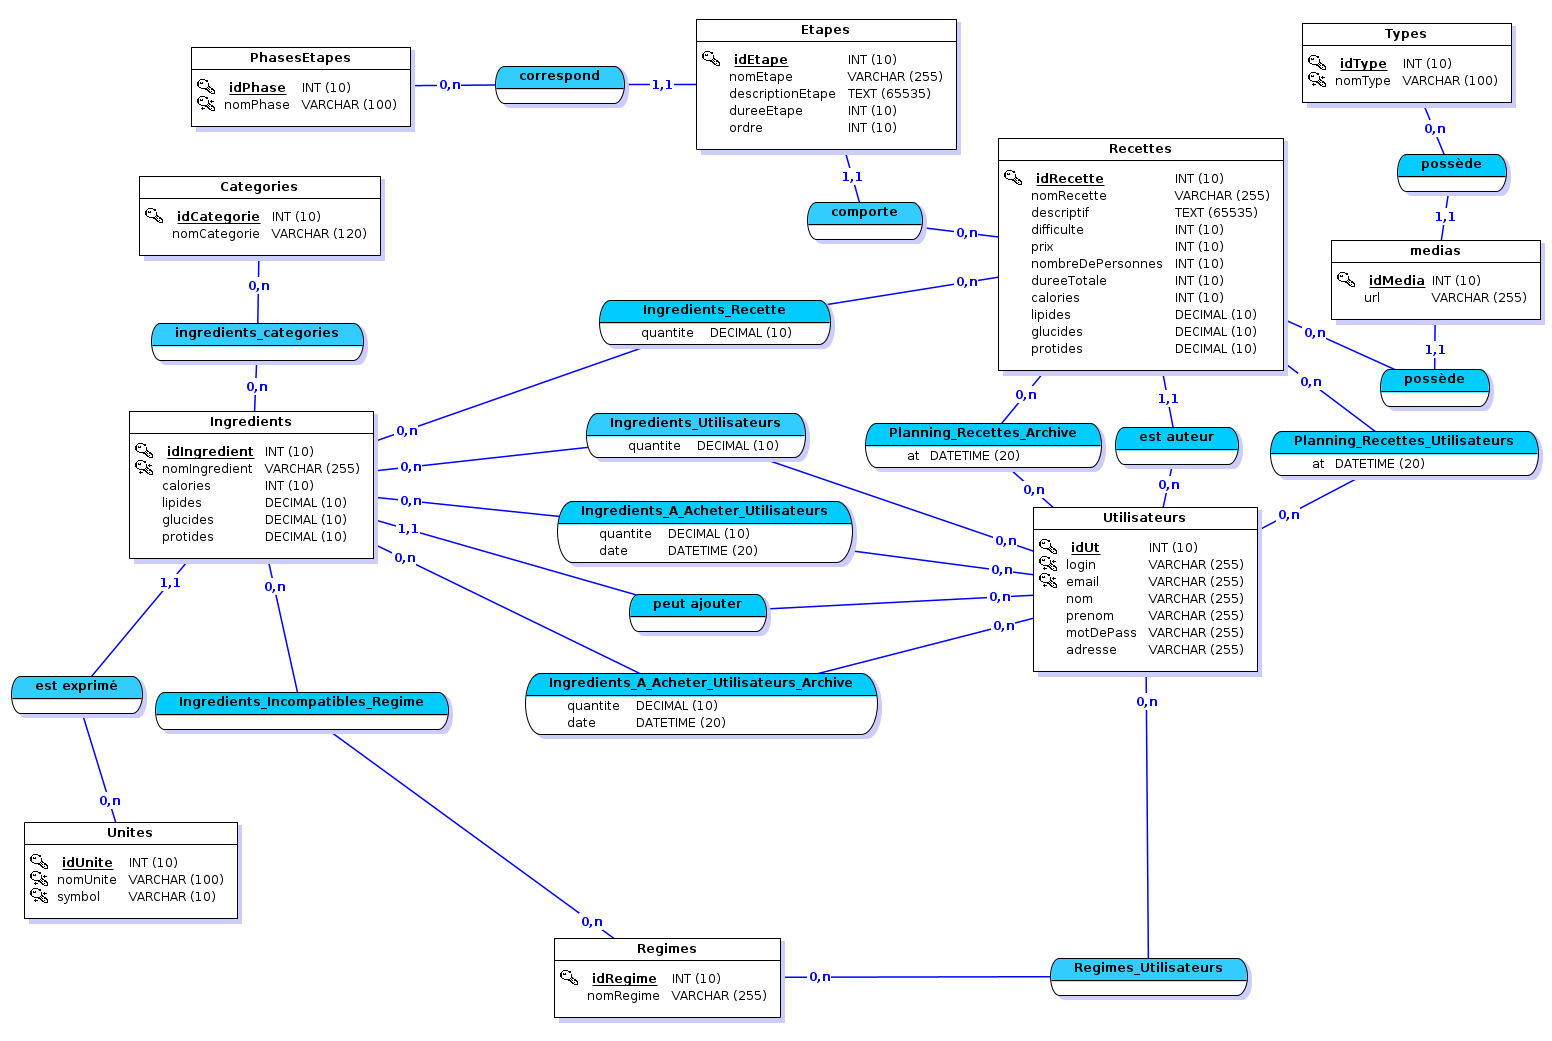
\includegraphics[scale=0.3]{images/RecetteDeCuisineJMerise.png}
    \caption{Modèle entité association.}
    \label{fig:modele E/A}
\end{figure}
Figure \ref{fig:modele E/A} shows MCD.

\subsection{La table Utilisateurs}
Elle receuillera l'ensembles des utilisateurs inscrits sur notre site web.
Un utilisateur est caractérisé par:
\begin{description}
    \item[idUt] Une clé primaire, numbre permettant d'identifier de façon unique un utilisateur.
    \item[login] nom d'utilisateur permettant de se connecter à la base de données. Il est propre à chaque users donc unique.
    \item[email] une adresse mail sur lequel on pourra le joindre. Elle est unique.
    \item[nom] contenant son nom patrimonial. Il peut être renseigner par l'utilisateur ou non.
    \item[prenom] contenant son prénom. Peut lui aussi être vide.
    \item[motDePass] le mot de pass de l'utilisateur. Elle sera necessaire pour se logger. Cette information étant sensible, sera crypée avant stockage en interne à l'aide d'un hash du type \textbf{sha1} ou autre variante.
    \item[adresse] contiendra l'adresse postale de l'utilisateur.
\end{description}

\subsection{La table Ingredient}
Elle sera utile pour stocker l'ensemble des ingrédients disponibles. Un ingrédient est caractérisé par:
\begin{description}
    \item[idIngredient] clé primaire, numéro permettant d'indentifier de façon unique un ingrédient.
    \item[nomIngredient] le nom de l'ingrédient.
    \item[calories] le nombre de calories qu'il contient.
    \item[lipides] nombre décimal représentant la quantité de lipides.
    \item[glucides] nombre décimal représentant la quantité de glucides.
    \item[protides] nombre décimal représentant la quantité de protides.
\end{description}
\textbf{\textit{Quand est-il de l'unité ?}}
\newline
En effet, pour pouvoir exprimer la quantité d'un ingrédient, on aura besoin d'une unité de mesure. Cette unité dépendra du type d'ingrédient. On pourra par exemple dire: \textit{4 oeufs} ou \textit{250g de farine} etc. L'unité fera l'objet d'une table.
\newline
\textbf{\textit{Pourquoi donc ne pas se contenter d'un champ supplémentaire ?}}
\newline
Dans un premier temps, dans la spécification du sujet, il est indiqué que la quantité pourra être indiqué soit en unité, soit en gramme. Je trouve celà trop restreint en faisant une comparaison avec le monde réel. Dans une tel situation, il sera impossible d'utiliser par exemple le \textit{Litre} et se serait dommage.
\newline
En second lieu, celà faciliteraît l'ajout d'une nouvelle unité et donc une mise à jour des éléments présents sur notre site sans modifier à chaque fois le code \textit{HTML}. On pourra par exemple via un formulaire \textit{HTML} récuperer dynamiquement les unités présentes dans la BDD et donc les mettre à disposition de l'utilisateur.

\subsection{La table Unites}
Elle contiendra l'ensemble des unités disponibles. Une unité est caractérisé par:
\begin{description}
    \item[idUnite] numéro permettant d'identifier une unité.
    \item[nomUnite] le nom de l'unité. Elle est unique.
    \item[symbole] le symbole associé à cette unité. par exemple \textit{g pour gramme, kg pour kilogramme etc.}. Elle peut être \texttt{NULL} mais dans le cas contraire sera unique.
\end{description}

\subsection{La table Categorie}
Elle contiendra l'ensemble des Categorie ou type d'ingrédient disponibles. Par exemple: \textit{Poisson}. On pourra remplacer dans certaines recettes à base de poisson \textit{la lotte} par de \textit{la saumonette}. Elle est caractérisé par:
\begin{description}
    \item[idCategorie] numéro permettant d'identifier un type d'ingrédient
    \item[nomCategorie] Le nom de la categorie.
\end{description}

\subsection{La table Regimes}
Elle stock l'ensemble des régimes possibles pour un individu. Elle sra caractérisé par:
\begin{description}
    \item[idRegime] numéro permettant d'indentifier un régime particulier
    \item[nomRegime] le nom du régime. par exemple: \textit{Végétarien, Halal} etc.
\end{description}

\subsection{La table Recette}
Elle contiendra l'ensemble des recettes disponibles. Elle est caractérisé par:
\begin{description}
    \item[idRecette] numéro permettant d'identifier une recette en particulier.
    \item[nomRecette] le nom de la recette
    \item[descriptif] La description de la recette.
    \item[difficulte] une évaluation du type: \textit{Très facile, Facile, Intermédiaire, Difficile, Très difficile}.
    \item[prix] entier allant de \textit{1} à \textit{5} estimant le prix.
          \begin{itemize}
              \item 1: Gratuit
              \item 2: Bon marché
              \item 3: Prix moyen
              \item 4: élevé
              \item 5: Très élevé
          \end{itemize}
    \item[nombreDePersonne] entier représentant le nombre de personne pour lequel la recette est destinée. Ce nombre peut être ajusté au niveau du site web entrainant ainsi l'ajustement d'autres paramètres comme la quantité des ingrédients etc.
    \item[dureeTotal] un entier représentant la durée total exprimé en minute pour la réalisation de la recette.
    \item[calories] entier représentant le nombre de calories fournis par la recette.
    \item[lipides] nombre décimal indiquant la quantité global de lipides contenu dans la recette.
    \item[glucides] nombre décimal indiquant la quantité global de glucides
    \item[protides] nombre indiquant la quantité de global protides.
\end{description}

\subsection{La table Etape}
Elle contiendra l'ensemble des étapes à suivre pour la réalisation de la recette. Elle est caractérisé par:
\begin{description}
    \item[idEtape] numéro identifiant une Etape
    \item[nomEtape] nom de l'étape. par exemple: \textit{la sauce !}
    \item[descriptionEtape] une description détaillé de l'étape. par exemple:"\textit{Mélanger la crème à la moutarde. Ajoutez le sel et le poivre}"
    \item[dureeEtape] la durée de l'étape exprimé en minute.
    \item[ordre] entier d'indiquant le rang (ou la priorité) dans la suite des étape de réalisation d'une recette.
\end{description}

\subsection{La table phaseEtape}
Elle présente l'ensemble des phases relatives à aux différentes étapes. par exemple la phase de \textit{Cuisson, Péparation, Repos etc}. Elle est caractérisé par:
\begin{description}
    \item[idPhase] numéro identifiant une phase.
    \item[nomPhase] le nom de la phase.
\end{description}

\subsection{La table medias}
Elle stock l'ensemble des médias disponibles pour les recettes. Par exemple: \textit{photos, images, vidéos, audios etc}. Elle est caractérisé par:
\begin{description}
    \item[idMedia] numéro identifiant un média.
    \item[url] lien permettant d'accéder au média.
\end{description}

\subsection{La table types}
Elle présente les différents types de média disponibles. Par exemple: \textit{vidéo spot publicitaire, vidéo storytelling, vidéo tutoriel etc.}. elle est caractérisé par:
\begin{description}
    \item[idType] numéro identifiant le type de média
    \item[nomType] le nom du type de média.
\end{description}


\section{Les contraintes d'intégrité}
Pour garantir la cohérence du modèle précédant, les données doivent respecter à tout instant un certaines nombre de constraintes.
\newline
Les identifiants des tables sont des clés primaires et par définition doivent être \texttt{unique} et \texttt{non NULL}.

\subsection{La table Utilisateurs}
\begin{description}
    \item[login] est propre à chaque utilisateur, donc unique
    \item[email] doit être unique, doit respecter le format d'une adresse valide c'est-à-dire de la forme \texttt{[au\_moins\_un\_caractère]@[ au\_moins\_un\_caractère]}. Ce traitement pourra se faire dans un langage dynamique à l'instar de \textit{php} grâce aux \textit{régex}.
    \item[motDePass] doit être \texttt{non vide}.
    \item[nom] doit être \texttt{non vide}.
    \item[prenom] doit être \texttt{no vide}.
\end{description}

\subsection{La table Ingredients}
\begin{description}
    \item[nomIngredient] doit être \texttt{unique} et \texttt{non NULL}
    \item[calories] doît être positive ou null \(\geqslant 0\).
    \item[lipides] doît être positive ou null \(\geqslant 0\).
    \item[glucides] doît être positive ou null \(\geqslant 0\).
    \item[protides] doît être positive ou null \(\geqslant 0\).
\end{description}

\subsection{La table Unites}
\begin{description}
    \item[nomUnite] doit être \texttt{non NULL} et \texttt{unique}.
    \item[symbole] doit être \texttt{unique} mais peut être \text{NULL}. C'est le cas des ingrédients quantifiables par unité. Par exemple: \textit{oeufs}
\end{description}

\subsection{La table Categories}
\begin{description}
    \item[nomCategorie] doit être \texttt{unique, non NULL}.
\end{description}

\subsection{La table Regimes}
\begin{description}
    \item[nomRegime] doit être \texttt{unique, non NULL}.
\end{description}

\subsection{La table Recettes}
\begin{description}
    \item[nomRecette] doit être \texttt{non NULL}.
    \item[difficulte] doit appartenir à l'ensemble \{\textit{Très facile, Facile, Intermédiaire, Difficile, Très difficile}\}.
    \item[prix] doit être compris entre \texttt{1} et \texttt{5}.
    \item[nombreDePersonne] doît être positive ou null \(\geqslant 0\).
    \item[dureeTotale] doît être positive ou null \(\geqslant 0\).
    \item[calories] doît être positive ou null \(\geqslant 0\).
    \item[lipides] doît être positive ou null \(\geqslant 0\).
    \item[glucides] doît être positive ou null \(\geqslant 0\).
    \item[protides] doît être positive ou null \(\geqslant 0\).
\end{description}

\subsection{La table Etapes}
\begin{description}
    \item[nomEtape] doit être \texttt{non NULL}.
    \item[dureeEtape] doît être positive ou null \(\geqslant 0\).
    \item[ordre] doît être positive ou null \(\geqslant 0\).
\end{description}

\subsection{La table phasesEtapes}
\begin{description}
    \item[nomPhase] doit être \texttt{unique, non NULL}.
\end{description}

\subsection{La table medias}
\begin{description}
    \item[url] doit être \texttt{non NULL}.
\end{description}

\subsection{La table types}
\begin{description}
    \item[nomType] doit être \texttt{unique, non NULL}.
\end{description}

\section{Les relations}
Le modèle précédent présente un ensemble étiqueté d'entités chacune jouant un rôle particulier. Il s'agit des relations/liaisons indiquant les liens entres différentes tables. Les exemples suivantes explique la sémantique des liens entre les différentes tables.

\subsection{Liens entre la table Recette et Utilisateurs}
Un utilisateur inscrits dans la base de données peut créer et donc être l'auteur de \texttt{0} à \texttt{n} recettes et une recette est édité par \texttt{1} et \texttt{1} seul utilisateur.
\newline
Un utilisateur peut établir un planning contenant \texttt{0} à \texttt{n} recettes et une recette peut faire l'objet de \texttt{0} à \texttt{n} planning. Il faut donc par la suite créer une table \texttt{Planning\_Recettes\_Utilisateurs} qui établira la correspondance utilisateur (\textit{idUt}) et la recette (\textit{idRecette}) prévu dans son planning.
\newline
Comme il s'agit d'un planning, cette table devra contenir en plus un champ (\texttt{at}) de type \texttt{datetime} indiquant la date prévu pour cette recette.
Une des contraintes que devra respecter ce champ est que sa valeur dois être comprise entre l'instant \texttt{t} d'établissement du planning et les \texttt{n} prochains mois (\textit{n fixé par l'admin. Pour simplifier on supposera que n vaut 1}). 
\newline
Si cette date est dépassée, le planning sera archivé c'est-à-dire conservé dans une autre table \(\texttt{Planning\_Recettes\_Archive}\).

\subsection{Liens entre la table Recettes et Etapes}
Une recette peut comporter \texttt{0} (\textit{Si elle vient juste d\textquoteright être créer}) à \texttt{n} étapes. Par contre une étape est relative à une recette et donc est utilisée dans \texttt{1} et \texttt{1} seul recette.

\subsection{Liens entre la table Etapes et PhasesEtapes}
A une étape on peut faire conspondre \texttt{1} et \texttt{1} seul phase (\texttt{par exemple: le fait de couper les léguments corrspondre à la phase de préparation}) et une phase peut comporter \texttt{0} à \texttt{n} étapes différentes.

\subsection{Liens entre la table Recettes et Medias}
Une recette peut posséder \texttt{0} à \texttt{n} médias et un média référence à \texttt{1} et \texttt{1} seul recette.

\subsection{Liens entre la table Medias et Types}
Un média est d\textquoteright \texttt{1} et \texttt{1} seul type donné et un type de média peut regrouper \texttt{0} à \texttt{n} médias différents.

\subsection{Liens entre la table Recettes et Ingrédients}
Une recette est composé de \texttt{0} (\textit{si elle vient juste d\textquoterightêtre créée}) à \texttt{n} ingrédients et une recette peut être utlisée dans \texttt{0} à \texttt{n} recette.s . Il faut donc par la suite créer une table \texttt{Ingredients\_Recettes} qui établira la correspondance ingrédient (\textit{idIngredient}) et la recette (\textit{idRecette}) dans laquel elle est utilisée.
\newline
Dans cette table, Il faudrait disposer aussi d'un champ (\texttt{quantite}) de type décimal indiquant la quantité de cet ingrédient necessaire pour la recette.

\subsection{Liens entre la table Ingrédients et Categories}
Un ingrédient peut appartenir à \texttt{0} à \texttt{n} catégorie.s et une catégorie regroupe \texttt{0} à {n} ingrédients. Il faut donc par la suite créer une table \texttt{Ingredients\_Categories} qui établira la correspondance ingrédient (\textit{idIngredient}) et la categorie (\textit{idCategorie}) dans laquel elle appartient.

\subsection{Liens entre la table Ingrédients et Unites}
Un ingrédient est quantifié/mesusé à l'aide d'une \texttt{1} et \texttt{1} seul unité et une unité est utilisée pour mesurer \texttt{0} à \texttt{n} ingrédient.s. Il faut donc par la suite créer un champ dans la table \texttt{Ingredients} qui fera référence à \textit{idUnite} de la table \texttt{Unites}.

\subsection{Liens entre la table Ingrédients et Utilisateurs}
Un utilisateur peut disposer de \texttt{0} à \texttt{n} ingrédients et un ingrédient peut être possédé par \texttt{0} ou \texttt{n} utilisateur.s. Il faut donc par la suite créer une table \texttt{Ingredients\_Utilisateurs} qui établira la correspondance ingrédient (\textit{idIngredient}) et son possesseur (\textit{idUt}).
Dans cette table, Il faudrait disposer aussi d'un champ (\texttt{quantite}) de type décimal indiquant la quantité de cet ingrédient que possède l'utilisateur.
\newline
Un utilisateur pourra comparer la liste des ingrédients dont il dispose avec la liste des ingrédients nécessaires pour réaliser les recettes sur son planning. Dans ce cas il peut ajouter \texttt{0} à \texttt{n} ingrédient.s et un ingrédient est ajouté par \texttt{1} et \texttt{1} seul utilisateur. 
\newline
Il faut donc par la suite créer un champ dans la table \texttt{Ingredients} qui fera référence à \textit{idUt} de la table \texttt{Utilisateurs}.
\newline
En fonction des ingrédients qui lui manque, l'utilisateur pourra établir une liste d'achât. Un utilisateur peut donc acheter \texttt{0} à \texttt{n} ingrédient.s et un ingrédient peut faire l'objet d'un achât par \texttt{0} à \texttt{n} utilisateur.s. Il faut donc par la suite créer la table \texttt{Ingredients\_A\_Acheter\_Utilisateurs} qui établira la correspondance ingrédient (\textit{idIngredient}) et l'utilisateur (\textit{idUt}) qui l'achète.
\newline
Dans cette table, Il faudrait disposer aussi d'un champ (\texttt{quantite}) de type décimal indiquant la quantité de cet ingrédient que va acheter l'utilisateur ainsi qu'un champ (\texttt{date}) de type \texttt{datetime} indiquant la date d'âchat.
\newline
Une des contraintes que devra respecter le champ \textit{date} est que sa valeur dois être comprise entre l'instant \texttt{t} d'établissement de la liste d'âchat et les \texttt{n} prochains mois (\textit{n fixé par l'admin. Pour simplifier on supposera que n vaut 1}). 
\newline
Si cette date est dépassée, la liste sera archivé c'est-à-dire conservé dans une autre table \texttt{Ingredients\_-
A\_Acheter\_Utilisateurs\_Archive}.


\subsection{Liens entre la table Regimes et Utilisateurs}
Un régime peut être suivis par \texttt{0} à \texttt{n} utilisateur.s et un utilisateur peut suivre \texttt{0} à \texttt{n} régime.s. Il faut donc par la suite créer une table \texttt{Regimes\_Utilisateurs} qui établira la correspondance régime (\textit{idRegime}) et l'utilisateur (\textit{idRecette}) qui le suit.

\subsection{Liens entre la table Regimes et Ingrédients}
Un ingrédient peut être incompatible à \texttt{0} à \texttt{n} régime.s et un régime peut exclure \texttt{0} à \texttt{n} ingrédient.s. Il faut donc par la suite créer une table \texttt{Ingredients\_Incompatibles\_Regimes} qui établira la correspondance régime (\textit{idRegime}) et l'ingrédient (\textit{idIngredient}) exclut.

\section{Le modèle logique relationel}
Cette partie présente les différentes tables ainsi que l'ensemble des relations déduites du \textit{Modèle entité association}. voici donc le \textbf{modèle relationel} correspondant. Pour des questions de lisibilités, vous pouvez aussi vous référer au dossier \texttt{images/index.png}.

\begin{figure}
    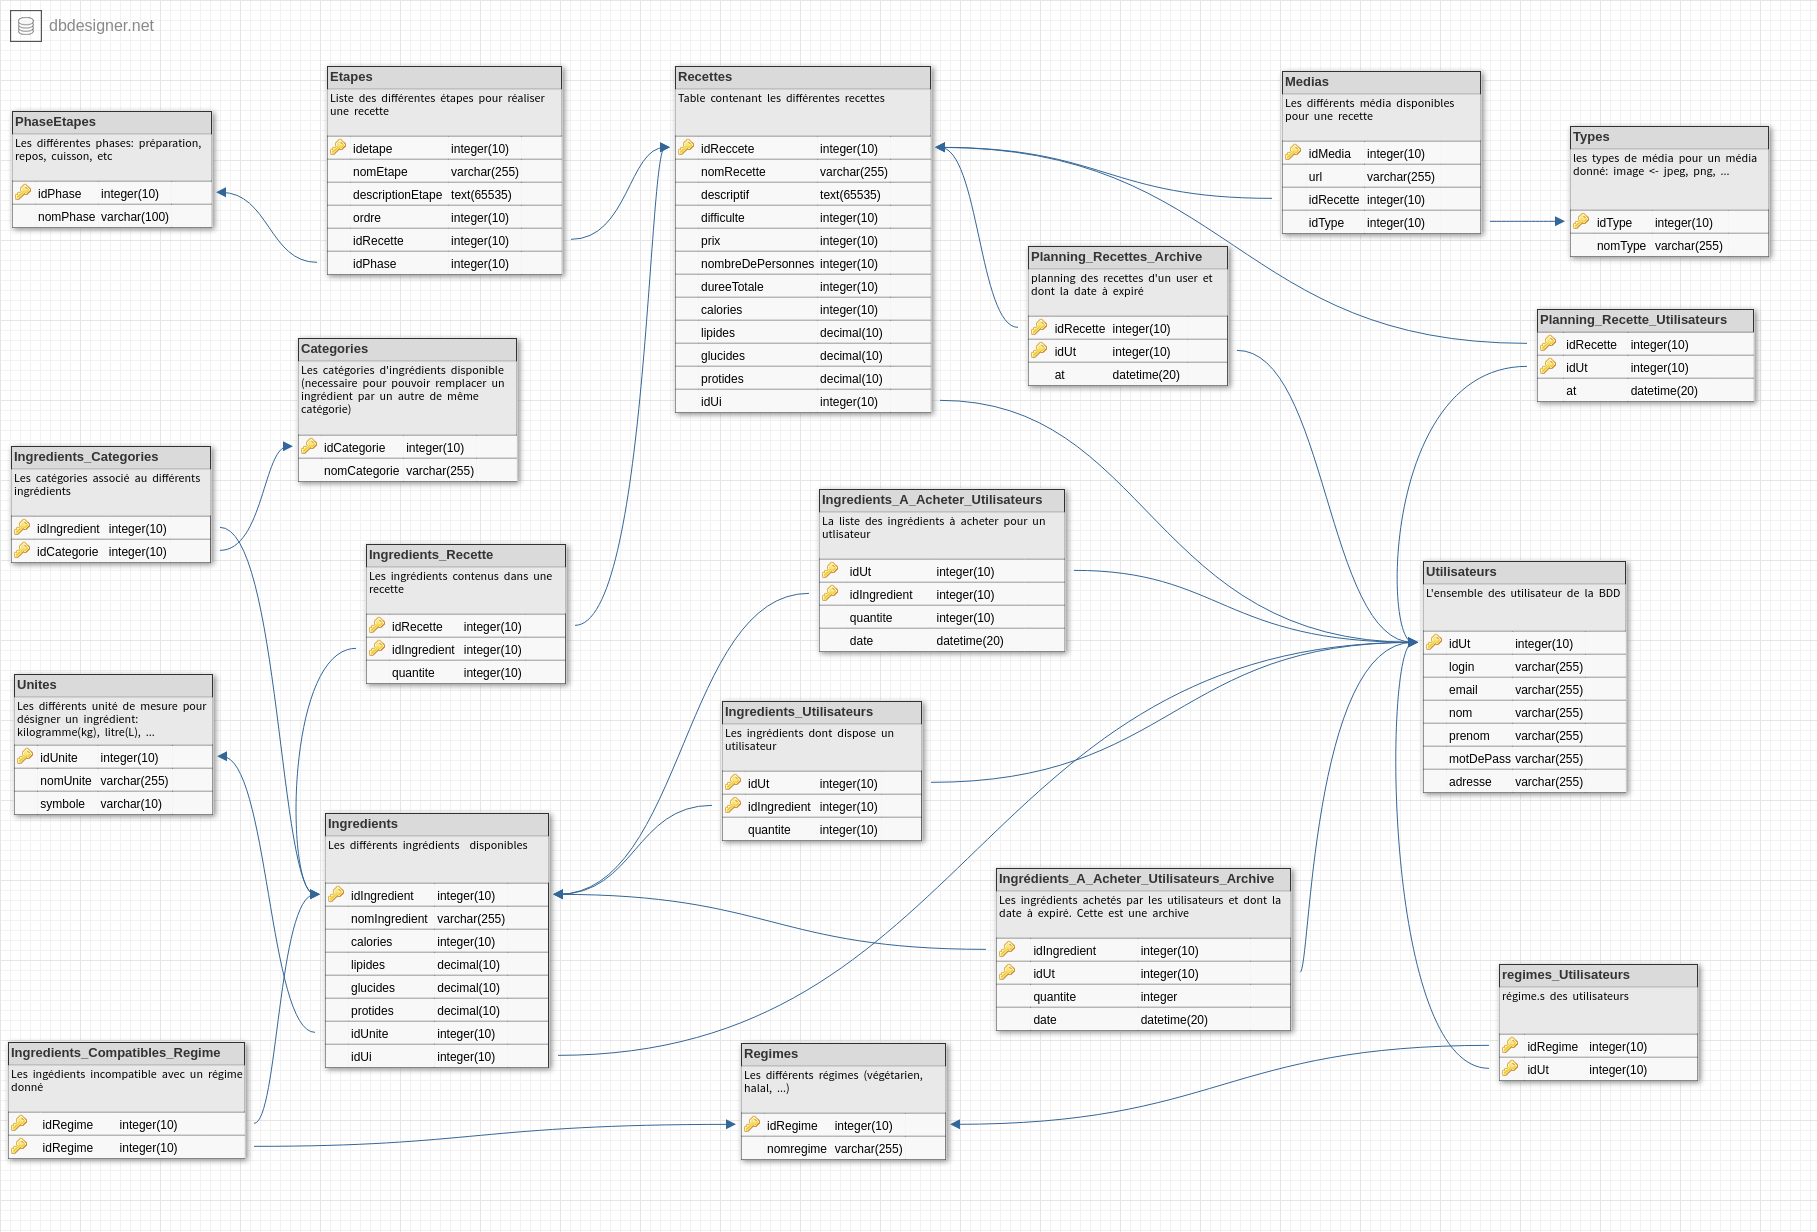
\includegraphics[scale=0.3]{images/index.png}
    \caption{Modèle logique relationel.}
    \label{fig:modele E/R}
\end{figure}
Figure \ref{fig:modele E/R} shows MLR.
\chapter{L'implémentation de la base données}

\section{Création des tables}
confert le repertoire \texttt{/requetes-pl-sql/\dots}

\section{Suppression des tables}
confert le repertoire \texttt{/requetes-pl-sql/\dots}

\section{Insertion de données}
confert le repertoire \texttt{/requetes-pl-sql/\dots}

\input{Chapitre3/Chapitre3}
%\chapter*{Conclusion g�n�rale}
\begin{thebibliography}{100}

\addtolength{\leftmargin}{0.2in}
\setlength{\itemindent}{-0.2in}

\bibitem{a} Marmiton. "\emph{Marmiton : 70000 recettes de cuisine ! Recettes commentées et notées pour toutes les cuisines.}" \textsc{Recette}. Dernière modification Mai 2020. (visité le 29 Octobre 2021). \textsc{url:} \href{https://www.marmiton.org/}{\texttt{\url{https://www.marmiton.org/}}}

\bibitem{b} Bastien, L. "\emph{Voici les 13 compétences nécessaires pour devenir data scientist}" \textsc{LeBigData}. Publié le 20 Juillet 2017. (visité le 07 Mars 2020) \textsc{url:} \href{http:/www.lebigdata.fr/13-competences-necessaires-devenir-data-scientist}{\texttt{\url{www.lebigdata.fr/13-competences-necessaires-devenir-data-scientist}}}

\end{thebibliography}
%\bibliographystyle{plain} 
\bibliography{Bibliographie/BibliographieBDD}
\addcontentsline{toc}{chapter}{Bibliographie}

%-----------------Fin Zone 5: fin de la num�rotation avec les chiffres arabs---------------------

\end {document}